\documentclass[referee]{aa} % for a referee version
%\documentclass[onecolumn]{aa} % for a paper on 1 column  
%\documentclass[longauth]{aa} % for the long lists of affiliations 
%\documentclass[letter]{aa} % for the letters 
%\documentclass[bibyear]{aa} % if the references are not structured 
%                              according to the author-year natbib style

%
%\documentclass{aa}  
\newcommand{\bea}{\begin{eqnarray}}
\newcommand{\eea}{\end{eqnarray}}
\newcommand{\ben}{\begin{enumerate}}
\newcommand{\een}{\end{enumerate}}
\newcommand{\bi}{\begin{itemize}}
\newcommand{\ei}{\end{itemize}}
\newcommand{\bmi}[1]{\begin{minipage}{#1 cm}}
\newcommand{\emi}{\end{minipage}}
\renewcommand{\[}{\begin{equation}}
\renewcommand{\]}{\end{equation}}

\renewcommand{\rm}{\mathrm}
\def\inv{^{-1}}
\def\({\left(}
\def\r){\right)}
\def\b#1{\bm{#1}}
\def\Dd{D_{\text{d}}}
\def\Dds{D_{\text{ds}}}
\def\Ds{D_{\text{s}}}
\def\la{\left<}
\def\ra{\right>}
\def\gammao{\gamma^{\text{obs}}}
\def\gammaoh{\hat{\gamma}^{\text{obs}}}
\def\epsilonsij{\epsilon_{a_i}\epsilon_{b_j}^*}
\def\epsilonsii{\epsilon_{a_i}\epsilon_{b_i}^*}
\def\deltafuncij{\Delta(\b\theta_{a_i}-\b\theta_{b_j})}
\def\d{\rm{d}}

%\newcommand{\todo}{\emph}

\usepackage{bm}
\usepackage{verbatim}
%
\usepackage{graphicx}
%%%%%%%%%%%%%%%%%%%%%%%%%%%%%%%%%%%%%%%%
\usepackage{txfonts}
%%%%%%%%%%%%%%%%%%%%%%%%%%%%%%%%%%%%%%%%
%\usepackage[options]{hyperref}
% To add links in your PDF file, use the package "hyperref"
% with options according to your LaTeX or PDFLaTeX drivers.
%
\usepackage{todonotes}

\begin{document} 


   \title{The Effects of Varying Depth in Cosmic Shear Surveys}

%   \subtitle{}

   \author{S. Heydenreich\inst{1}%\fnmsep\thanks{sven@astro.uni-bonn.de}
          \and Peter Schneider\inst{1} 
          \and Hendrik Hildebrandt\inst{2,1}
          \and Catherine Heymans\inst{3} 
          \and Marika Asgari\inst{3}
          \todo{order of authors?, KiDS-Authors?}
          }
   \institute{Argelander-Institut f\"ur Astronomie, Auf dem H\"ugel 71, 53121 Bonn, Germany 
\and 
Astronomisches Institut, Ruhr-Universit\"at Bochum, Universit\"atsstr. 150, 44801 Bochum, Germany \and
Institute for Astronomy, University of Edinburgh, Royal Observatory, Blackford Hill, Edinburgh EH9 3HJ, UK  \\ \email{sven@astro.uni-bonn.de}
             }

   \date{Received XXX; accepted XXX}

  \abstract
% context (optional)
   {Cosmic shear proves to be a powerful tool to study the properties of the local Universe. The discrepancy in the parameter $S_8$ between measurements in the local Universe and the Cosmic Microwave Background motivates further investigation of yet unaccounted systematic biases. 
% aims
   Especially ground-based surveys are subject to a variation in depth. We want to understand and quantify the resulting effects. In particular, we check if they introduce a bias to the cosmological parameters and if they can be responsible for the occurence of $B$-Modes.
% methods
   We construct a semi-analytic model to estimate the impact on the shear correlation function and analyze the implications for cosmological parameters. Furthermore we construct COSEBIs of the correlation functions to quantify the occuring B-Modes.
% results
   For the Kilo-Degree Survey this effect introduces an error in $\xi_\pm$ of the order of a few percent on small scales, which is responsible for a $0.1\sigma$ bias in $\Omega_{\rm m}$ and $\sigma_8$. However, the parameter $S_8$ is robust against this modification. We also report the occurrence of B-Modes, although not to a significant degree.
% conclusions (optional)
   We conclude that the effects of varying optical depth for ground-based surveys on cosmological parameters are not yet significant, but should be accounted for in next-generation experiments.}

   \keywords{gravitational lensing --
                weak lensing --
                cosmic shear
               }

   \maketitle

%
%-------------------------------------------------------------------

\section{Introduction}
The discovery of cosmic shear has provided us with a new and powerful cosmological tool to investigate the $\Lambda$CDM Model and determine its parameters. Contrary to the analysis of the Cosmic Microwave Background \citep{2018arXiv180706209P}, cosmic shear is more sensitive to the properties of the local Universe and thus provides an excellent consistency check for the standard model of cosmology. Current Cosmic Shear surveys are especially sensitive to the paramter $S_8=\sigma_8 \sqrt{\Omega_{\rm m}/0.3}$, where $\sigma_8$ denotes the normalisation of the matter power spectrum and $\Omega_{\rm m}$ is the matter density.
It is interesting to note that all three current major cosmic shear results report a lower $S_8$ than inferred from CMB analysis: While \citet{2018arXiv180706209P} determined a value of $S_8 = 0.830 \pm 0.013$, 
%\citet{2013MNRAS.432.2433H} report $S_8 = 0.759 \pm 0.020$ from analysis of CFHTLens data,
\citet{2018arXiv180909148H} report $S_8 = 0.800^{+0.029}_{-0.028}$ from analysis of the Subaru Hyper Suprime-Cam survey, \citet{2017MNRAS.465.1454H} report $S_8 = 0.745\pm 0.038$ from KiDS data and the Dark Energy Survey \citep{2018PhRvD..98d3528T} reports $S_8=0.782\pm 0.027$. Also, \citet{2013MNRAS.432.2433H} report $S_8 = 0.759 \pm 0.020$ from analysis of CFHTLens data. This discrepancy could be a statistical coincidence, a sign of new physics or the manifestation of an unknown systematic effect. \todo{Citations.. \citet{2017MNRAS.464.1676A} has a few...}

To check for remaining systematics, a weak lensing signal can be divided into two components, the so-called E- and B-modes \citet{2002ApJ...568...20C,2002A&A...389..729S}. To leading order, B-modes can not be created by astrophysical phenomena and are thus an excellent test for remaining systematics. As \citet{2017MNRAS.465.1454H} report the significant detection of B-modes, it is well motivated to check for possible systematics that are yet unaccounted for. Note that the non-existence of B-modes does not imply that the sample is free of remaining systematics.

One systematic effect is the variation of depth in a survey. While effects like Galactic extinction or dithering strategies do play a role in every survey, this work focuses on the effects caused by varying atmospheric conditions, that are found in ground-based surveys. To first order, this variation can be modelled by a step-like depth function that varies from pointing to pointing. In this work we assume the specifications of the Kilo-Degree Survey, namely a collection of $1\,\text{deg}^2$ square fields. Furthermore we neglect boundary effects. 

In Section \ref{sec:modelling_single_lens} we will introduce a simple toy model to understand this effect and analyze the impact on the power spectrum. In Section \ref{sec:xipm} we will estimate the effect on the shear correlation functions $\xi_\pm$ using two different models. We will present our results in Section \ref{sec:results}. In Section \ref{sec:discussion} we will discuss our results and comment on the impacts of our used simplifications. We will assume the standard weak gravitational lensing formalism, a summary of which can be found in \citet{2001PhR...340..291B}.

\section{Modelling the Power Spectrum}
\label{sec:modelling_single_lens}
For our first analysis we will further simplify our assumptions: We imagine that all the matter between sources and observer is concentrated in a single lens plane of distance $D_{\rm d}$ from the observer. If we now distribute sources at varying distances $D_{\rm s}$, then the convergence $\kappa$ varies according to $\kappa \propto D_{\rm ds}/D_{\rm s}$. 
% Following \citet{1993ApJ...404..441K}, we can simulate the shear $\gamma$ from the convergence by convolution with the kernel \[
%\mathcal{D}(\bm{\theta}) = \frac{\theta_2^2-\theta_1^2-2i\theta_1\theta_2}{\pi |\bm{\theta}|^4}\, .
%\]

%Similarly, an observer that measures the shear $\gamma$ can reconstruct the convergence $\kappa$ by convolution with the kernel $\mathcal{D}^*$, where ${}^*$ denotes the complex conjugate. Assuming that the optical depth, and thus the source redshift populations, vary between pointing, an observer will measure a shear-signal that is modified by a depth-function $W(\bm{\theta}) = 1-w(\bm{\theta})$, where $\langle w(\bm{\theta})\rangle=0$ holds. The reconstruction of the observed convergence $\kappa^{\rm obs}$ will thus not yield the original convergence. In particular there is no reason why the convolution with a complex kernel should have a nonzero imaginary part. This allows us to separate our received signal into E- and B-modes following \[
%	\kappa = \kappa^E+i\kappa^B\, ,
%\]
%where $B$-Modes can not be generated by a lensing signal and are thus a tracer of remaining systematics.
%2002A&A...389..729S SRC

\subsection{Effects on the Power Spectrum}
Assuming that the depth, and thus the source redshift populations, vary between pointings, an observer will measure a shear-signal that is modified by a locally constant depth-function $\gammao(\b\theta)=W(\b \theta)\gamma(\b\theta)$ with $W(\bm{\theta}) = 1+w(\bm{\theta})$, where $\langle w(\bm{\theta})\rangle=0$ holds. 
In accordance to the definition of the shear power spectrum \begin{equation}
(2\pi)^2\delta(\b\ell-\b\ell')P(|\b\ell|) = \la \hat{\gamma}(\b\ell)\hat{\gamma}(\b\ell')\ra \, ,
\end{equation}
we define the observed power spectrum via \begin{equation}
P^{\text{obs}}(\b\ell) \equiv \frac{1}{(2\pi)^2}\int \d^2 \ell'\,  \la \gammaoh(\b \ell) \gammaoh {}^*(\b \ell')\ra \, .
\end{equation}
Note that due to the depth-function both the assumptions of homogeneity and isotropy break down, which means that we can neither assume isotropy in the power spectrum, nor can we assume that $\la \gammaoh(\b \ell) \gammaoh {}^*(\b \ell')\ra$ vanishes for $\b\ell\neq\b\ell'$.
To model a constant depth on each individual pointing $\b \alpha$, we can choose random variables $w_{\b \alpha}$, that only need to satisfy $\langle w_{\b \alpha}\rangle=0$, and parametrize $w(\b\theta)$ as 
\begin{equation}
w(\b \theta) = \sum_{\b \alpha \in \mathbb{Z}^2} w_{\b \alpha} \Xi(\b \theta-L\b \alpha)\text{ , with the Box-Function } \Xi(\b \theta) = \begin{cases}
1 \qquad \b \theta\in \left[-\frac{L}{2},\frac{L}{2}\right]^2 \\
0 \qquad \text{else}
\end{cases},
\label{eq:defweightf}
\end{equation}
where $L$ is the length of one pointing.
Following the calculations in Appendix \ref{sec:calc of PS}, we derive 
\begin{equation}
P^{\text{obs}}(\b \ell)  =  P(\b \ell) + \la w^2\ra \int\frac{\text{d}^2\b k}{(2\pi)^2}\,\hat{\Xi}(\b \ell-\b k)P(\b k)\, ,
\end{equation}
where $\la w^2\ra \equiv \la w_{\b \alpha}^2\ra$ is the dispersion of the depth-function.
The observed power spectrum $P^{\text{obs}}$ is thus composed of the original power spectrum $P$, plus a convolution of the power spectrum with the fourier transfrom of a box-function, scaling with the variance of the geometric lensing efficiency $\la \frac{D_{\rm ds}}{D_{s}}\ra$. In particular, the power spectrum is not isotropic anymore. Following \citet{2002A&A...389..729S}, it would be interesting to extract E- and B-mode information out of this power spectrum, however \citet{2010A&A...520A.116S} present a more sophisticated decomposition of E- and B-modes, that can also be applied to real data using the shear correlation function, so instead we want to focus our efforts on these parts.
\section{Modelling the shear correlation function}
\label{sec:xipm}
A convenient way to infer cosmological information from observational data are the shear correlation functions $\xi_\pm$, which are defined as \[
\xi_\pm = \la \gamma_{\rm t}\gamma_{\rm t}\ra \pm \la \gamma_\times\gamma_\times\ra \, .
\]
They are the prime estimators to quantify a cosmic-shear signal since it is simple to include a weighting of the shear-measurements into the correlation functions and, contrary to the power spectrum, one does not have to worry about the shape of the survey footprint, or masked regions. Cosmologically, given two comoving distance probability distributions of sources $p_i(\chi),p_j(\chi)$, one can compute the shear correlation function from the underlyting matter power spectrum $P_\delta$ via \todo{Citation!}\begin{align}
\label{eq:xipm-pkappa}
\xi_\pm[\theta,p_i,p_j] =& \int_0^\infty \frac{{\rm d}l\,l}{2\pi}J_{0,4}(l\theta)P(l,p_i,p_j)\, , \\
\label{eq:pkappa-pdelta/lenseff}
P(l,p_i,p_j) =& \frac{9 H_0^4\Omega_{\rm m}^2}{4c^4}\int_0^{\chi_h} {\rm d}\chi\frac{g(\chi,p_i)g(\chi,p_j)}{a^2(\chi)}P_\delta\left(\frac{l}{f_K(\chi)},\chi\right)\, , \\
\label{eq:lenseff}
g(\chi,p_i) =& \int_\chi^{\chi_H} {\rm d}\chi'\, p_i(\chi') \frac{f_K(\chi'-\chi)}{f_K(\chi')}\, .
\end{align}
Here, $J_{0,4}$ denote the 0-th and 4-th order Bessel Functions.
\subsection{Using an analytic Model}
For a first simple analysis we will assume that a deeper redshift distribution just yields a stronger shear signal. Following \citet{2006APh....26...91V}, we estimate
\[
\la |\gamma| \ra \propto \la z \ra ^{0.85}\, .
\]
\todo{Maybe implement redshift-dependent index?}
Additionally, we assume that a higher depth does not only lead to a stronger average shear, but also to a higher galaxy number density, implying a correlation between those two quantities.

%For a pair of galaxies that we use to measure the correlation function, it is crucial to determine whether those two galaxies lie within the same pointing. We want to define a function $E(\theta)$ that determines 

Let $N(\b \theta)$ be the number-density per tile and $W(\b \theta)$ the weighting of average shear. The observed correlation function $\xi^{\text{obs}}_\pm(\theta)$ now changes from one of constant depth $\xi_\pm^{\rm const}$ via 
\begin{align*}
\xi^{\text{obs}}_\pm(\theta) = & \frac{\la N(\b 0)N(\b \theta)\gammao_{\rm t}(\b 0)\gammao_{\rm t}(\b \theta)\ra }{\la N(\b 0)N(\b \theta)\ra} \pm \frac{\la N(\b 0)N(\b \theta)\gammao_\times(\b 0)\gammao_\times(\b \theta)\ra }{\la N(\b 0)N(\b \theta)\ra} \\
 = & \frac{\la N(\b 0)N(\b \theta)W(\b 0)W(\b \theta)\ra}{\la N(\b 0)N(\b \theta)\ra} \xi_{\pm}^{\rm const}(\theta) \, .
 \end{align*}
 Assuming that depth and galaxy number density of neighbouring pointings are uncorrelated, the only important property of a galaxy pair is whether or not they lie in the same pointing. We want to denote the probability that a random pair of galaxies of distance $\theta$ lie in the same pointing with $E(\theta)$. An analytical expression for this function is surprisingly hard to obtain, but it can easily be calculated to arbitrary accuracy, following the procedure explained in Appendix \ref{sec:details on etheta}. The function is depicted in Figure \ref{fig:eoftheta_lin}. 
 
 \begin{figure}
 \centering
 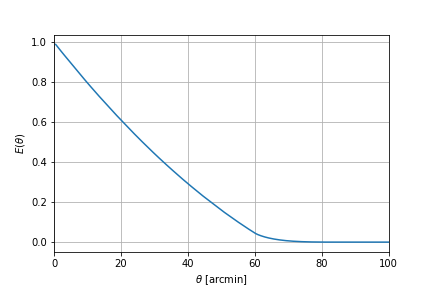
\includegraphics[width=0.5\textwidth]{images/eoftheta.png}
 \caption{Probability that a random pair of galaxies of distance $\theta$ lie in the same pointing.}
 \label{fig:eoftheta_lin}
 \end{figure}

We again parametrize the number density $N(\b \theta)=\la N \ra (1+n(\b \theta))$ and the weight $W(\b \theta)=1+w(\b \theta)$ and, as in \eqref{eq:defweightf}, interpret $n(\b \theta)$ as a locally constant function with average $\la n \ra = 0$. We can see that $\la n(\b 0)n(\b \theta)\ra = E(\theta)\la n(\b 0)n(\b 0)\ra \equiv E(\theta)\la n n \ra$ holds and get
 \begin{align}
\xi^{\text{obs}}_\pm(\theta) = & \frac{1 + 2\la nw \ra + E(\theta)\left[\la (n+w)^2\ra + 2 \la n^2 w\ra + 2\la nw^2\ra + \la n^2 w^2\ra \right]}{1+E(\theta)\la n^2\ra }\xi_\pm^{\rm const}(\theta) \\
\approx & \frac{1 + 2\la nw \ra + E(\theta)\left[\la (n+w)^2\ra \right]}{1+E(\theta)\la n^2\ra }\xi_\pm^{\rm const}(\theta)\, . \nonumber
 \label{eq:ffunct}
\end{align}
\todo{The formula for a cross-correlation of different bins is much longer, but follows the same principle. Maybe put it into the Appendix?}
We see that in addition to a modification of the correlation function due to the stronger shear signal in deeper pointings, we also get a scale-independent modification due to the correlation between depth and number density.

However, as a survey of constant depth is completely unrealistic, also the modelled correlation function will be subject to the same effect. If we assume the same redshift-distributions for galaxies as in the case of varying depth, and just assert that those changes are not correlated with position, we get 
\begin{equation}
\xi_\pm = (1+2\la nw\ra)\xi_\pm^{\rm const}\, .
\end{equation}
The ratio of modelled and observed correlation function thus becomes: \begin{align}
\frac{\xi_\pm}{\xi_\pm^{\rm obs}} = & \frac{\left(1+2\la nw\ra\left)\left(1+E(\theta)\la n^2\ra\right)\right.\right.}{1 + 2\la nw \ra + E(\theta)\left[\la (n+w)^2\ra + 2 \la n^2 w\ra + 2\la nw^2\ra + \la n^2 w^2\ra \right]} \\
\equiv & F(\theta) \, .
\end{align}
%It is interesting to note that $F(\theta)=1$ holds wherever $E(\theta)=0$, meaning that the correlation function is not affected for large angular scales. 
We shall later see that this approximation is valid for higher tomographic redshift bins $z\gtrsim 0.5$, but starts to break down at lower redshifts. 
\subsection{Using a semi-analytic Model}
The analysis of data from the Kilo-Degree Survey showed that the redshift-distribution of sources was highly correlated with the depth in the $r$-band. We thus chose to separate the survey into 10 percentiles, sorted by $r$-band depth, meaning that if a pointing had a worse depth than 90\% of the other pointings, it would belong to the first percentile, and so on. Now for each percentile $i$ and each tomographic redshift bin $z$ we can extract a weighted number density of galaxies $N_i(z)$ and, in case the pointing overlaps with a spectroscopic survey, a source redshift distribution $p_i(z)$. Using \eqref{eq:xipm-pkappa}, we can for each set of percentiles $i,j$ and redshift bins $z_1,z_2$ compute the shear correlation function $\xi_\pm[\theta,p_i(z_1),p_j(z_2)]$.\todo{Should we cite \textsc{nicaea} here?} When we compute the measured shear correlation function of a survey, we take the weighted average of tangential and cross shears of all pairs of galaxies (\citet{2017MNRAS.465.1454H} give a good overview for the process). If, for a single pair of galaxies, one galaxy lies in the $i$-th percentile of redshift bin $z_1$ and the second one lies in the $j$-th percentile of redshift bin $z_2$, then their contribution to the observed correlation function is, on average, $\xi_\pm[\theta,p_i(z_1),p_j(z_2)]$. This means that if we know each of those single correlation functions, we can reconstruct the total correlation function via a weighted average of the single functions. As an example, if we want to calculate the correlation function between tomographic bins $z_1$ and $z_2$ and pick a galaxy from bin $z_1$, the probability of this galaxy being in the $i$-th percentile of $z_1$ is proportional to $N_i(z_1)$. Now let the second galaxy be in bin $z_2$ and of distance $\theta$ to the first. If we imagine a thin annulus of radius $\theta$ around the first galaxy, then the number of galaxies in this annulus, that lie within the same pointing as the first galaxy, is proportional to $E(\theta)N_i(z_2)$, whereas the number of galaxies that lie in a different pointing is $[1-E(\theta)]\la N(z_2)\ra$, where $\la N(z_2)\ra$ is the average number density in redshift bin $z_2$. If the galaxy lies within a different pointing, the chances of it being in the $j$-th percentile are again just proportional to $N_j(z_2)$. We conclude that if we sum the single correlation functions $\xi_\pm[\theta,p_i(z_1),p_j(z_2)]$ according to these weightings, we can simulate the observed correlation function that accounts for the variation in optical depth via 
\begin{align}
\xi_{\pm,z_1,z_2}^{\rm obs}(\theta) = & \frac{1}{C}\sum_{i=1}^{10} N_i(z_1) \bigg\{ E(\theta) N_i(z_2) \xi_\pm\big[\theta,p_i(z_1),p_i(z_2)\big] + \la N(z_2)\ra\sum_{j=1}^{10}\frac{  N_j(z_2)}{\sum_k N_k(z_2)} \big[1-E(\theta)\big]\xi_\pm\big[\theta,p_i(z_1),p_j(z_2)\big]\bigg\} \nonumber \\
 = & \frac{1}{C}\sum_{i=1}^{10} N_i(z_1) \bigg\{ E(\theta) N_i(z_2) \xi_\pm\big[\theta,p_i(z_1),p_i(z_2)\big] + \sum_{j=1}^{10}\frac{1}{10} \big[1-E(\theta)\big] N_j(z_2)\xi_\pm\big[\theta,p_i(z_1),p_j(z_2)\big]\bigg\}\, ,
\label{eq:correctionfunction1}
\end{align}
with the normalization
\[
C = \sum_{i=1}^{10} N_i(z_1) \bigg[ E(\theta)  N_i(z_2) + \sum_{j=1}^{10} \frac{1}{10} \big[1-E(\theta)\big] N_j(z_2)\bigg]\,.
\]
A more mathematically rigorous derivation of this function can be found in Appendix \ref{sec:calc of xipm}.
If we want to compute this for all 5 redshift bins of the KiDSV-survey, this forces us to calculate 1265 correlation functions and add them, thus yielding potential numerical errors (apart from being computationally expensive). However, if we examine Equation \eqref{eq:lenseff}, we see that it is linear in its second argument, which in turn makes Equations \eqref{eq:pkappa-pdelta/lenseff} and \eqref{eq:xipm-pkappa} bilinear in their second and third arguments. This basically means that, instead of adding correlation functions, we can add their respective redshift distributions and compute the correlation function of that. As an example, the following equation holds: \[
N_j\xi_\pm[\theta,p_i,p_j]+N_k\xi_\pm[\theta,p_i,p_k] = (N_j+N_k)\,\xi_\pm\left[\theta,p_i,\frac{N_jp_j+N_kp_k}{N_j+N_k}\right]\, .
\]
Consequently, we can apply this to \eqref{eq:correctionfunction1}, yielding
\begin{equation}
\xi_{\pm,z_1,z_2}^{\rm obs}(\theta) = \frac{1}{C}\bigg\{ E(\theta)\sum_{i=1}^{10} N_i(z_1)N_i(z_2) \xi_\pm\big[\theta,p_i(z_1),p_i(z_2)\big] +\frac{1}{10}\big[1-E(\theta)\big]\xi_\pm\left[\theta,p(z_1),p(z_2)\right]N(z_1)N(z_2)\bigg\}\, .
\label{eq:correctionfunction2}
\end{equation}
Here, we defined the \textit{average redshift distribution} $p(z)$ and \textit{combined number density} $N(z)$ of tomographic bin $z$ as \[
p(z):= \frac{\sum_i N_i(z)p_i(z)}{\sum_i N_i(z)}\, , \qquad N(z):=\sum_i N_i(z)\, .
\]
\todo{Maybe label the $N(z)$ differently to avoid confusion with $\la N(z)\ra$?}
For each set of redshift bins we thus only have to compute eleven correlation functions, which reduces the number of functions to compute from 1275 to 165. We can see that for large distances $\theta$, such that $E(\theta)=0$ holds, we have $C=N(z_1)N(z_2)$ and thus \[
\xi_{\pm,z_1,z_2}^{\rm obs}(\theta) = \frac{1}{N(z_1)N(z_2)}\xi_\pm\left(\theta,n(z_1),n(z_2)\right)N(z_1)N(z_2) = \xi_{\pm,z_1,z_2}(\theta)\, ,
\]
so on large scales our observed correlation function agrees with the one that we would usually calculate.
\section{Results}
\label{sec:results}
We applied both our methods to data from the KiDSV-450 survey and computed the ratio of observed and modeled correlation functions. Furthermore, we have conducted a simulation using ray-tracing through the millenium simulations (?)\todo{I should ask catherine about what exactly she did for the simulations or maybe even ask her to write this part of the paper?}. As in \citet{2018arXiv181206076H}, we have separated the data in 5 tomographic redshift bins and performed our analysis for a cross-correlation of all bins. The result can be seen in Figure \ref{fig:all_xis}.
	\begin{figure}
	\centering
	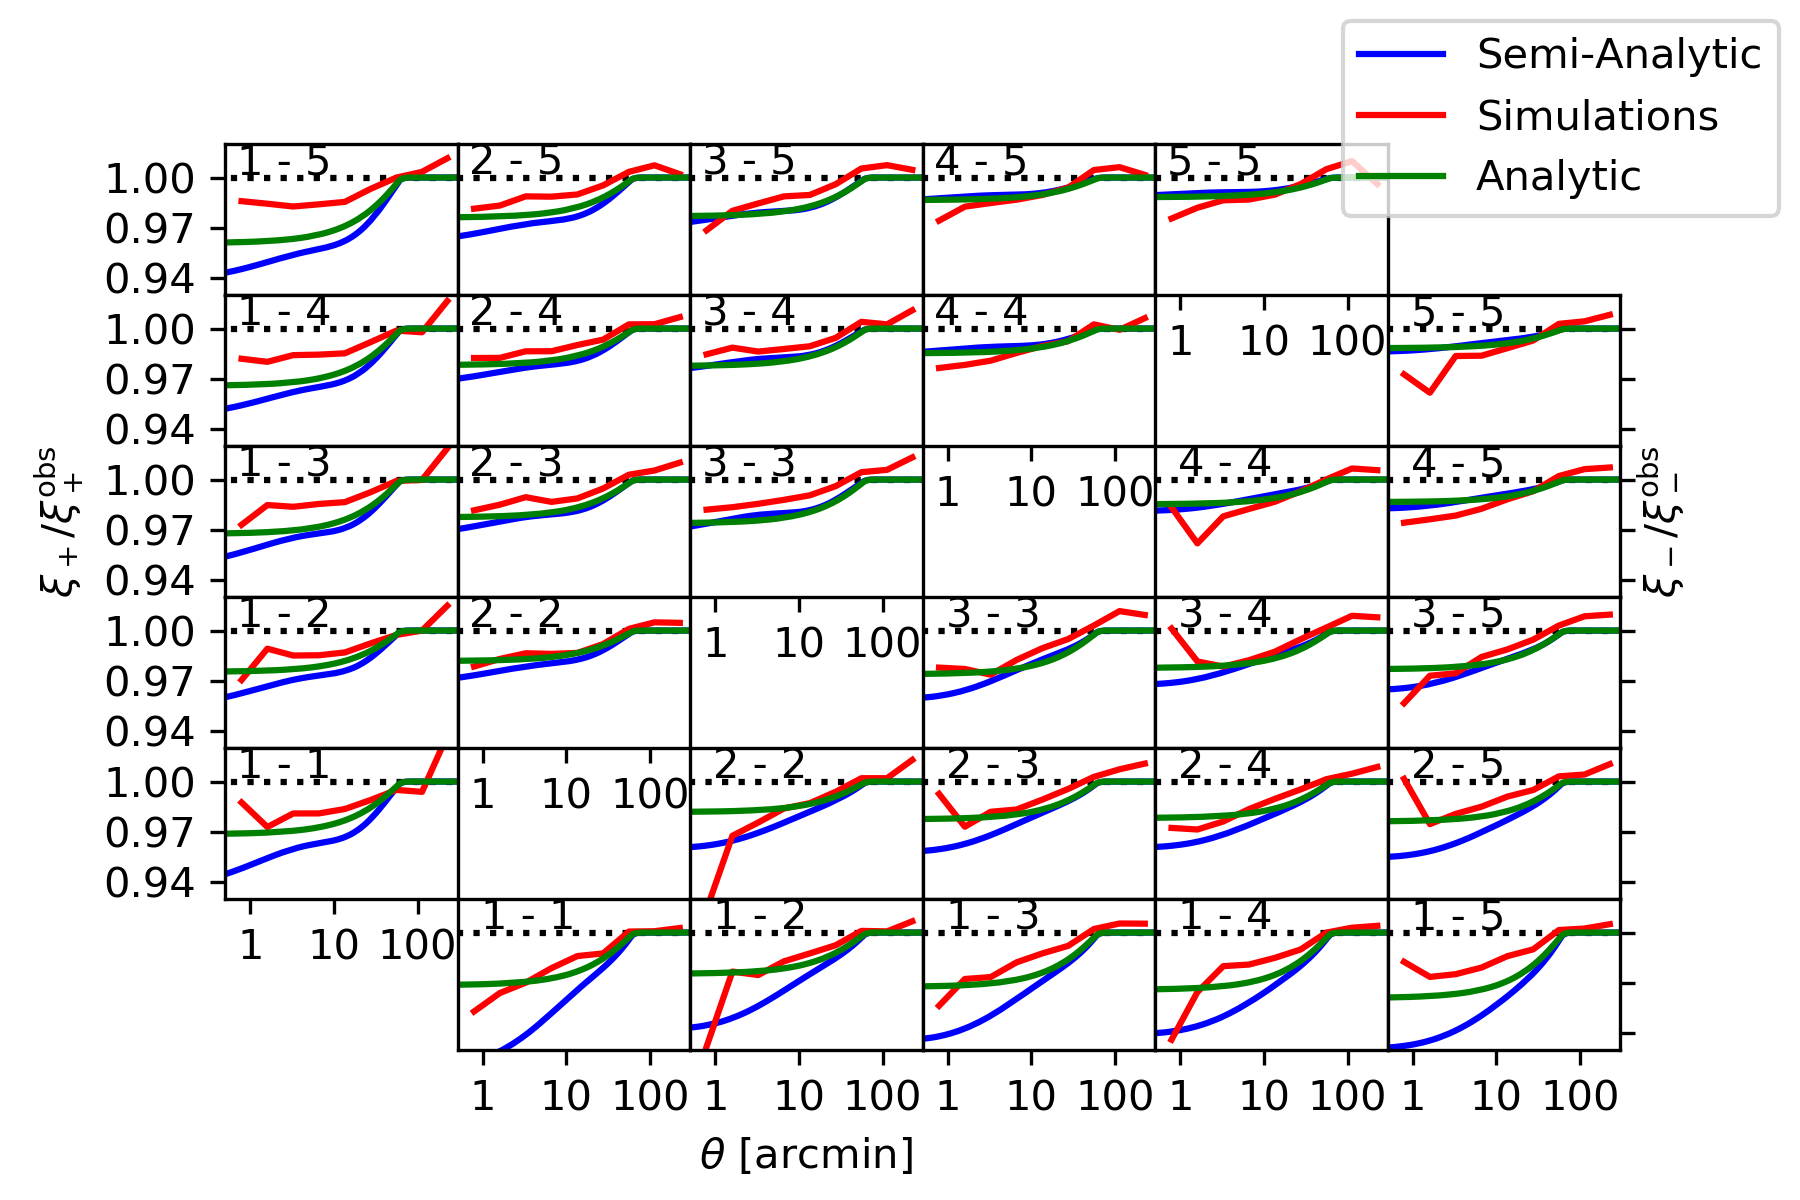
\includegraphics[width=1\textwidth]{images/xis_111.png}
	\caption{The ratio of observed to modeled correlation functions for the analytic method (green), the semi-analytic method (blue) and the numerical simulations (red) for a cross-correlation of all redshift bins.}
	\label{fig:all_xis}
	\end{figure}
We can see that for high redshift bins, the analytic and the semi-analytic methods are consistent, whereas for low redshift bins they significantly diverge. We explain this due to the facts that the analyic method uses simplifications that are redshift-dependent and only hold for small variations in redshift, which is not fulfilled in the low redshift bins.\todo{Should I include the plot number density vs average redshift from the talk? Maybe in the appendix to avoid too many Figures?} The simulations seem to be in rough agreement with the models, but there are some features that can not be explained. Especially we observe that the ratios of the correlation functions for large values of $\theta$ seem to consistently surpass unity, which can not be explained by our models.

As the next step we computed a reference correlation function given a fiducial cosmology for each combination of redshift bins, and modified said correlation function according to our semi-analytic model. Then we ran a Markov-Chain Monte Carlo simulation\footnote{The code for this was developed by Jan-Luca van den Busch and used in a modified version.} to check for a potential bias in the cosmological parameters, using the covariance-matrix computed in \citet{2017MNRAS.465.1454H}. As our main interest lies in the $\Omega_{\rm m}$ - $\sigma_8$ combination, we restricted our analysis to those two parameters.\todo{Maybe expand this to more parameters?}  As can be seen in Figure \ref{fig:mcmc_kids}, the impact of varying depth is noticeable, but insignificant compared to the uncertainties. However, to get a rough estimate for the impact on a Euclid-like survey, we divided the used covariance-matrix by 30, to account for the increased survey area. As can be seen in Figure \ref{fig:mcmc_euclid}, here the impact on both $\Omega_{\rm m}$ and $\sigma_8$ is significant, however it seems that the parameter $S_8$ is extremely robust against this effect.

To estimate the B-Modes created by this effect, we have extracted the \emph{Complete Orthogonal Sets of E- and B-Mode Integrals} (COSEBIS, compare \citet{2010A&A...520A.116S}), once of a reference set of correlation functions, to estimate numerical inaccuracies,\footnote{For a reference correlation function the B-Modes should be consistent with zero.} and then for the correlation functions that have been modified to account for a varying depth. We report a consistent B-Mode pattern across all redshift-bins, which can be seen in Figure \ref{fig:bmodes_cosebi}. Although we did not determine the error bars, that a KiDS-like survey would imply on those functions, \citet{2018arXiv181110596A} calculated the COSEBIs of the KiDSV-450 survey for the same range in $\theta$. The real B-Modes were about one order of magnitude higher than the ones created by the varying depth, and still found to be not significant. Given these facts, we conclude that the creation of B-Modes due to varying depth in the KiDS survey is not significant. However, the pattern seems to be very characteristic, so when one encounters B-Modes in next generation surveys, that show a similar pattern, this would suggest that they are created by a similar effect (although we can not exclude other effects that just create the same B-Mode pattern).

\begin{figure}
\centering
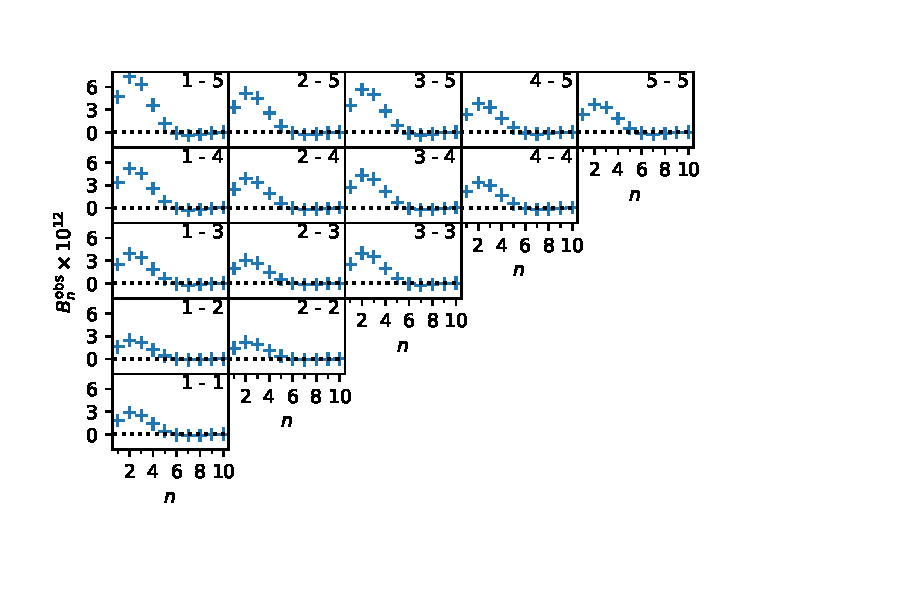
\includegraphics[width = \textwidth, trim = {0 1.5cm 2.5cm 0}, clip]{images/bmodes.pdf}
\caption{The $B$-modes created by a variation in survey-depth. We used the logarithmic COSEBIs described in \citet{2010A&A...520A.116S} with a range from $\theta_{\rm min} = 0.5\arcmin$ to $\theta_{\rm max} = 100\arcmin$.}
\label{fig:bmodes_cosebi}
\end{figure}

\section{Discussion}
\label{sec:discussion}
With our semi-analytic model we try to describe the impacts of varying depth in ground-based surveys. During our analysis we have assumed a few simplifications, which we will discuss.
\begin{enumerate}
\item We implemented a variation in depth that only depends on the pointing. However, in reality galactic extinction, CCD imperfections, dithering strategies and other factors also influence the depth on different scales. Although the variation between pointings is the dominating factor, a complete analysis implementing those factors could yield a slightly different result.
\item In our main analysis we assumed an infinite number of fields. This ignores boundary effects that would arise in the vincinity of the edge of a footprint (there finding a galaxy outside of the same pointing would be less likely). Also, another effect is ignored: If one has a number of $N$ fields in each percentile, and one galaxy is in a pointing of a certain percentile, then the probability that a different pointing is of the \emph{same} percentile is reduced by the factor $(N-1)/N$. However, we modeled the second effect, and already at 100 pointings it barely makes any difference. We did not model the boundary effects, but we assume that they are likewise neglible. \todo{This needs to be rewritten to account for the new insights.}
\item We have assumed that the depth of neighbouring pointings is uncorrelated. While there is no reason not to assume that, we have not yet verified that this is indeed the case.
\item In our Monte Carlo simulations we have only had $\Omega_{\rm m}$ and $\sigma_8$ as free parameters. While we do not expect most other parameters to make a difference, baryonic feedback and/or intrinsic alignments also change the correlation functions on small scales, so it is definitely possible that in a Monte Carlo chain including free parameters for these effects, those would change to mitigate the varying depth, and the impact on the actual cosmological parameters would be much smaller.
\end{enumerate}
We have determined that the effects of varying depth are not significant for the KiDSV-450 survey. For a Euclid-like survey they will play an important role, but before a model is implemented in such a precise survey, one should revise the used simplifications, especially the first one. We suspect that it should be possible to account for different aspects of varying optical depth by just modifying the function $E(\theta)$.

However, for the parameter $S_8$ this effect is insignificant, which in particular means that a variation in depth can not explain the discrepancies between the analyses of the CMB and those of the local universe. It can also be responsible for the occurence of $B$-Modes, although only to an insignificant amount.

%--------------------------------------------------------------------


\begin{acknowledgements}
Something should probably be put in here...
\end{acknowledgements}


\bibliographystyle{aa}
\bibliography{cite}
\begin{appendix}
\section{Detailed Calculations}
\subsection{Calculation of the Power Spectrum}
In this Section we will perform the calculation for the observed power spectrum \todo{I need to add cdots for scalar products in this section...} $P^{\text{obs}}(\b \ell)$. For this, we assume an infinitely large field in order to perform our integration over $\mathbb{R}^2$. In reality, finite field effects would play a role here. We begin with the calculation of the correlation for the Fourier transformed shear:
\begin{align}
\la \gammaoh(\b \ell) \gammaoh {}^*(\b \ell')\ra = & \la\int\text{d}^2\b \theta\int\text{d}^2\b \theta'\,W(\b \theta)W(\b \theta')\gamma(\b \theta)\gamma^*(\b \theta')\exp(i\b \ell\b \theta-i\b \ell'\b \theta')\ra\nonumber\\
 = & \la\int\text{d}^2\b \theta\int\text{d}^2\b \theta'\,W(\b \theta)W(\b \theta')\exp(i\b \ell\b \theta-i\b \ell'\b \theta') \int \frac{\text{d}^2\b k}{(2\pi)^2}\int \frac{\text{d}^2\b k'}{(2\pi)^2}\, \hat{\gamma}(\b k)\hat{\gamma}^*(\b k')\exp(-i\b k\b \theta+i\b k'\b \theta')\ra \nonumber\\
= & \la \int \text{d}^2\b \theta \int \text{d}^2\b \theta' \int \frac{\text{d}^2\b k}{(2\pi)^2} \int \frac{\text{d}^2\b k'}{(2\pi)^2}\, P(\b k)(2\pi)^2 \delta(\b k-\b k') \exp[i(\b \ell\b \theta-\b \ell'\b \theta'-\b k\b \theta+\b k'\b \theta')]W(\b \theta)W(\b \theta')\ra \nonumber\\
  = & \la \int \frac{\text{d}^2\b k}{(2\pi)^2} \, P(\b k) \int \text{d}^2\b \theta\, W(\b \theta)\exp[i\b \theta(\b \ell-\b k)]\int \text{d}^2\b \theta'\, W(\b \theta') \exp[-i\b \theta(\b \ell'-\b k)] \ra \nonumber\\
  = & \la \int\frac{\text{d}^2 \b k}{(2\pi)^2} \, P(\b k)\widehat{W}(\b \ell-\b k)\widehat{W}^* (\b \ell'-\b k)\ra
\end{align}
It is important to keep in mind that the ensemble averages of the weight function are independent of the ensemble averages of the shear values, meaning $\la W(\b \theta)\gamma(\b \theta)\ra = \la W(\b \theta)\ra \la \gamma(\b \theta)\ra$. We can define $W(\b \theta)=1+w(\b\theta)$ with $\la w(\b \theta)\ra = 0$, which leads to the expession
\begin{align}
\la \gammaoh(\b \ell) \gammaoh {}^*(\b \ell')\ra = & \la \int\frac{\text{d}^2 \b k}{(2\pi)^2} \, P(\b k) \left[ (2\pi)^4\delta(\b \ell-\b k)\delta(\b \ell'-\b k)+(2\pi)^2\big( \hat{w}(\b \ell-\b k)\delta(\b \ell'-\b k) + \hat{w}^*(\b \ell'-\b k)\delta(\b \ell-\b k)\big)\right.\right. \nonumber\\
 & \qquad \left.\left. + \hat{w}(\b \ell-\b k)\hat{w}(\b \ell'-\b k) \right] \right. \bigg> \nonumber\\
 = & (2\pi)^2\delta(\b \ell-\b \ell')P(\b \ell) + \big[ \la \hat{w}(\b \ell-\b \ell')\ra P(\b \ell')+\la \hat{w}^*(\b \ell'-\b \ell)\ra P(\b \ell)\big] + \la \int \frac{\text{d}^2 \b k}{(2\pi)^2} \, \hat{w}(\b \ell-\b k)\hat{w}^*(\b \ell'-\b k)P(\b k)\ra \nonumber\\
\overset{(*)}{=} & (2\pi)^2\delta(\b \ell-\b \ell')P(\b \ell) + \la \int \frac{\text{d}^2 \b k}{(2\pi)^2}\, \hat{w}(\b \ell-\b k)\hat{w}^*(\b \ell'-\b k)P(\b k)\ra \, ,
\label{eq:pobs1}
\end{align}
where in $(*)$ we have used that the average $\la \hat{w}(\b \ell)\ra$ vanishes.
Up until now, we have not specified our weight-function $w$. So we now parametrize it as \begin{equation}
w(\b \theta) = \sum_{\b \alpha \in \mathbb{Z}^2} w_{\b \alpha} \Xi(\b \theta-L\b \alpha)\text{ , with the Box-Function } \Xi(\b \theta) = \begin{cases}
1 \qquad \b \theta\in \left[-\frac{L}{2},\frac{L}{2}\right]^2 \\
0 \qquad \text{else}
\end{cases}.
\end{equation}
Here, the $w_{\b \alpha}$ are random variables, drawn from the random distribution describing the survey depths. For the Fourier-Transform we compute: \begin{equation}
\hat{w}(\b \ell) = \sum_{\b \alpha \in \mathbb{Z}^2} w_{\b \alpha} \exp(-i \b \ell L\b \alpha) \widehat{\Xi}(\b \ell)\, ,
\end{equation}
where
\begin{equation}
\widehat{\Xi}(\b\ell) = \frac{4\sin\left(\frac{L\ell_1}{2}\right)\sin\left(\frac{L\ell_2}{2}\right)}{\ell_1\ell_2}\, ,
\end{equation}
is a 2-dimensional sinc function.
Assuming an uncorrelated weight-distribution $\left(\la w_{\b \alpha} w_{\b \beta}\ra = 0\text{ for }\b \alpha\neq\b \beta\right)$ and setting $\la w^2\ra \equiv \la w_{\b \alpha}^2\ra$ for each $\b \alpha$, we get
\begin{align}
\la \int \frac{\text{d}^2 \b k}{(2\pi)^2}\, \hat{w}(\b \ell-\b k)\hat{w}^*(\b \ell'-\b k)P(\b k)\ra = & \la \int \frac{\text{d}^2 \b k}{(2\pi)^2} \sum_{\b \alpha,\b \beta}w_{\b \alpha}w_{\b \beta} \exp[-i(\b \ell - \b k)L\b \alpha]\, \widehat{\Xi}(\b \ell - \b k) \exp[i(\b \ell' - \b k)L\b \beta]\, \widehat{\Xi}^*(\b \ell' - \b k)P(\b k)\ra \nonumber\\
 = & \int \frac{\text{d}^2 \b k}{(2\pi)^2} \sum_{\b \alpha} \la w^2\ra \exp[-i(\b \ell - \b k)L\b \alpha + i(\b \ell' - \b k) L\b \alpha]\, \widehat{\Xi}(\b \ell - \b k)\widehat{\Xi}^*(\b \ell' - \b k)P(\b k) \, .
\end{align}
Using this result, we can obtain the observed power spectrum \begin{equation}
P^{\rm{obs}}(\b\ell) = \frac{1}{(2\pi)^2}\int\d^2\ell' \la \gammaoh(\b \ell) \gammaoh {}^*(\b \ell')\ra\, ,
\end{equation}
by performing the $\b \ell'$-integration in \eqref{eq:pobs1}:
\begin{align}
P^{\text{obs}}(\b \ell) = & P(\b \ell)+\int \frac{\text{d}^2\b \ell'}{(2\pi)^2} \int\frac{\text{d}^2\b k}{(2\pi)^2}\sum_{\b \alpha}\la w^2\ra \exp[-i(\b \ell-\b k)L\b \alpha+i(\b \ell'-\b k)L\b \alpha]\, \widehat{\Xi}(\b \ell-\b k)\widehat{\Xi}(\b \ell' - \b k) P(\b k) \nonumber\\
= & P(\b \ell)+ \int\frac{\text{d}^2\b k}{(2\pi)^2}\sum_{\b \alpha}\la w^2\ra \exp[-i(\b \ell-\b k)L\b \alpha]\, \widehat{\Xi}(\b \ell - \b k)P(k) \int\frac{\text{d}^2\b \ell}{(2\pi)^2}\, \widehat{\Xi}^*(\b \ell'-\b k)\exp[i(\b \ell'- \b k)L\b \alpha] \nonumber\\
 = & P(\b \ell) + \la w^2\ra \int\frac{\text{d}^2\b k}{(2\pi)^2}\, \widehat{\Xi}(\b \ell-\b k)P(\b k) \sum_{\b \alpha}\exp[-i(\b \ell - \b k)L\b \alpha]\,\Xi(L\b \alpha) \nonumber\\
 = & P(\b \ell) + \la w^2\ra \int\frac{\text{d}^2\b k}{(2\pi)^2}\,\widehat{\Xi}(\b \ell-\b k)P(\b k)\, ,
\end{align}
which is a 2-dimensional convolution of the power spectrum and the 2-dimensional sinc function.
\label{sec:calc of PS}
\subsection{Details on the function $E(\theta)$}
\label{sec:details on etheta}
The function $E(\theta)$ is of central importance in this model, so we want to explain how to obtain it. It describes, given a pair of galaxies with distance $\theta$, the probability that they are in the same pointing. We obtain the function in the following way:

Given one square field of length 1 and a separation vector $\b\theta$, without loss of generality we can assume $\theta_1,\theta_2\geq 0$. As depicted in Figure \ref{fig:explain_etheta}, the dashed square represents all possible positions that the first galaxy can take, such that the second galaxy is still within the same pointing. The volume of this square equals \begin{equation}
\tilde{V}(|\b\theta|,\phi)  = \big[1-|\b\theta|\cos(\phi)\big]\,\big[1-|\b\theta|\sin(\phi)\big]\, ,
\end{equation} where $\phi$ represents the angle of the vector $\b\theta$. To exclude negative Volumes (which would occur when $|\b\theta|>1$ holds), we nead to add the Heaviside theta function $H$:
\begin{equation}
V(|\b\theta|,\phi)  = \big[1-|\b\theta|\cos(\phi)\big]\,\big[1-|\b\theta|\sin(\phi)\big] H\big[1-|\b\theta|\cos(\phi)\big]\,H\big[1-|\b\theta|\sin(\phi)\big]\, .
\label{eq:eoftheta1}
\end{equation} 
To obtain the function $E(\theta)$, we need to average Equation \eqref{eq:eoftheta1} over all angles $\phi$. While the case $\theta_1,\theta_2\geq 0$ certainly does not hold for all angles $\phi$, we can eliminate the other cases by simple symmetry.
\begin{align}
E(\theta) = & \frac{4}{2\pi}\int_0^{\frac{\pi}{2}}\d\phi\, V(|\b\theta|,\phi) = \frac{2}{\pi}\begin{cases}
\int_0^{\frac{\pi}{2}} \d\phi\, \big[1-|\b\theta|\cos(\phi)\big]\,\big[1-|\b\theta|\sin(\phi)\big]\, , & |\b\theta|\leq 1 \\
\int_{\arccos(|\b\theta|^{-1})}^{\arcsin(|\b\theta|^{-1})} \d\phi\, \big[1-|\b\theta|\cos(\phi)\big]\,\big[1-|\b\theta|\sin(\phi)\big]\, , \quad & 1\leq |\b\theta| \leq \sqrt{2} \\
0\, , & \sqrt{2}\leq\theta
\end{cases} \nonumber\\
 = & \begin{cases}
\frac{\pi + (\theta-4)*\theta}{\pi}\, , & \theta \leq 1 \\
\frac{2[-1+2\sqrt{1-\theta^{-2}}*2\theta - \theta^2/2 - \arccos(\theta^{-1}) + \arcsin(\theta^{-1})]}{\pi}\, , & 1\leq \theta \leq \sqrt{2} \\
0\, , & \sqrt{2}\leq \theta
\end{cases}\, .
\end{align}
\begin{figure}
    \centering
    \def\svgwidth{200pt}    
    \input{images/eoftheta_new.pdf_tex}  
    \caption{Graphic representation on how to obtain the function $E(\theta)$. For a separation vector $\b\theta$, the dashed square represents the area of galaxies that have their partner in the same pointing.}
    \label{fig:explain_etheta}
\end{figure}
\subsection{Calculation of the shear correlation functions}
\label{sec:calc of xipm}
Following \citet{2017MNRAS.465.1454H}, given a set of galaxies we calculate the shear correlation function via \begin{equation}
\xi_+(\theta) = \frac{\sum_{a,b}w_aw_b\epsilon_a\epsilon_b^*\Delta(\b\theta_a-\b\theta_b)}{\sum_{a,b}w_aw_b\Delta(\b\theta_a-\b\theta_b)}\, .
\label{eq:xip_from_observations}
\end{equation}
Here, $w$ represents the lensing weight of the galaxy, whereas $\epsilon$ is its (complex) ellipticity and $\b \theta$ its position on the sky. We have defined the function $\Delta$ as \[
\Delta(\b\theta_a-\b\theta_b) = \begin{cases}
1, \,\, & |\b\theta_a-\b\theta_b| \in [\theta,\theta+{\rm d}\theta] \\
0, & \text{ else}
\end{cases}\, ,
\]
where we assume ${\rm d}\theta \ll \theta$. When we now separate our galaxy samples into the ten percentiles $I$ defined above, and denote the galaxies from sample $a$ that are in pointing $i$ with $a_i$, the numerator in Equation \eqref{eq:xip_from_observations} transforms to:
\begin{align*}
 & \sum_{i,j=1}^{10} \sum_{a_i,b_j} w_{a_i}w_{b_j}\epsilon_{a_i}\epsilon_{b_j}^*\Delta(\b\theta_{a_i}-\b\theta_{b_j}) \\
 = & \sum_{i=1}^{10}\sum_{a_i}w_{a_i} \sum_{j=1}^{10} \sum_{b_j} w_{b_j}\epsilon_{a_i}\epsilon_{b_j}\Delta(\b\theta_{a_i}-\b\theta_{b_j}) \\
 = & \sum_{i=1}^{10}\sum_{a_i}w_{a_i} \left[ \sum_{j=1}^{10} \sum_{b_j\in P_{a_i}} w_{b_j} \Delta(\b\theta_{a_i}-\b\theta_{b_j})\epsilonsij + \sum_{j=1}^{10}\sum_{b_j\not\in P_{a_i}} w_{b_j} \Delta(\b\theta_{a_i}-\b\theta_{b_j})\epsilonsij \right]
\end{align*}
We take the ensemble average of that equation in the sense that we assume that the product of the ellipticities of the galaxies are equal to their respective shear correlation functions, namely $\xi_+^{ij}\equiv \epsilon_{a_i}\epsilon_{b_j}^*$ for all $a_i$ and $b_j$.

Let $b_j\in P_{a_i}$ denote all $b_j$ that lie in the same pointing as the $a_i$. We observe that the left term is zero for $i\neq j$, as only galaxies of the same percentile can lie in the same pointing. The term $\sum_{b_i\in P_{a_i}}\deltafuncij$ now is the number of galaxies that lie within distance interval $[\theta,\theta+{\rm d}\theta]$ of galaxy $a_i$, which is equal to the number of galaxies in the whole pointing multiplied by $2\pi\theta\, {\rm d}\theta\, E(\theta)$. The prefactor $w_{b_i}$ transforms the number of galaxies to the \emph{weighted number density} of galaxy sample $b$ in percentile $i$, or $N_i(b)$, so the numerator now reads:
\begin{align*}
\sum_{i=1}^{10}\sum_{a_i}w_{a_i} \left[ 2\pi\theta\, {\rm d}\theta\, E(\theta) N_i(b)\xi_+^{ii} + \sum_{j=1}^{10}\sum_{b_j\not\in P_{a_i}} w_{b_j} \Delta(\b\theta_{a_i}-\b\theta_{b_j})\xi_+^{ij} \right]
\end{align*}

 A similar argument can be made for the right term: Assuming for a second that all pointings outside of the one where galaxy $a_i$ is in are of percentile $j^*$, the right hand side would read \[
\sum_{b_{j^*}\not\in P_{a_i}} w_{b_{j^*}} \Delta(\b\theta_{a_i}-\b\theta_{b_{j^*}})\xi_+^{i{j^*}} = 2\pi\theta\, {\rm d}\theta\, [1-E(\theta)]N_{j^*}(b)\xi_+^{i{j^*}}\, .
 \]  
 Taking the ensemble average of all realisations of depth-distributions, we can just denote the probability that a pointing neighbouring one of percentile $i$ is of percentile $j$ as $P(j | i,\theta)$. The numerator then reads \[
 \sum_{i=1}^{10}\sum_{a_i}w_{a_i} \left[ 2\pi\theta\, {\rm d}\theta\, E(\theta) N_i(b)\xi_+^{ii} + \sum_{j=1}^{10} P(j|i,\theta)\, 2\pi\theta\, {\rm d}\theta\, [1-E(\theta)]N_{j}(b)\xi_+^{i{j}} \right]\, .
 \]
 In our case we assume an infinite number of randomly distributed fields, so $P(j | i,\theta)=1/10$ holds. However, for a finite survey the footprint of depth-distributions seems to be of importance, as due to a limited number of fields the $P(j | i,\theta)$ does not equate its expectation value. For smaller surveys (or surveys with correlated depth-distributions) it seems appropriate to adjust this parameter. \todo{Wait for catherines 450deg${}^2$ simulations, maybe they are big enough?}
 
 If we define $A$ as the (arbitrarily big) survey area, we can set \[
 \sum_{a_i} w_{a_i} = A\, N_i(a)
 \]
 and see that the numerator becomes \[
 2\pi\theta\, {\rm d}\theta\, A \sum_{i=1}^{10}N_i(a) \left[E(\theta) N_i(b)\xi_+^{ii} + \sum_{j=1}^{10} P(j|i,\theta) [1-E(\theta)]N_{j}(b)\xi_+^{i{j}} \right]\, .
 \]
 The exact line of argumentation can be applied to the denominator, which then reads: \[
  2\pi\theta\, {\rm d}\theta\, A \sum_{i=1}^{10}N_i(a) \left[E(\theta) N_i(b) + \sum_{j=1}^{10} P(j|i,\theta) [1-E(\theta)]N_{j}(b) \right]\, .
 \]
Taking the ratio of the two quantities, and setting $P(j | i,\theta)=1/10$, we receive Equation \eqref{eq:correctionfunction1}.
\section{Additional Figures}
\subsection{Results of the MCMC}
\begin{figure}[h]
\centering
	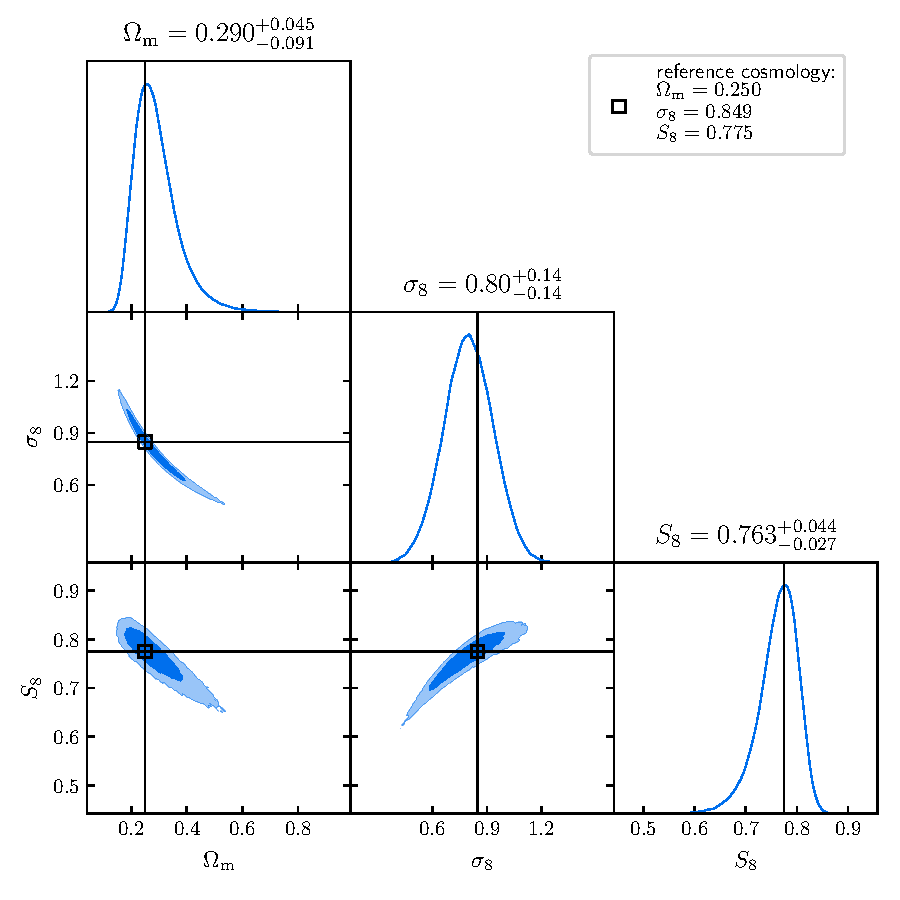
\includegraphics[width=0.7\textwidth]{images/obscorr.pdf}
	\caption{Bias in the parameters for a KiDS-like Survey.}
	\label{fig:mcmc_kids}
\end{figure}  
\begin{figure}[h]
\centering
	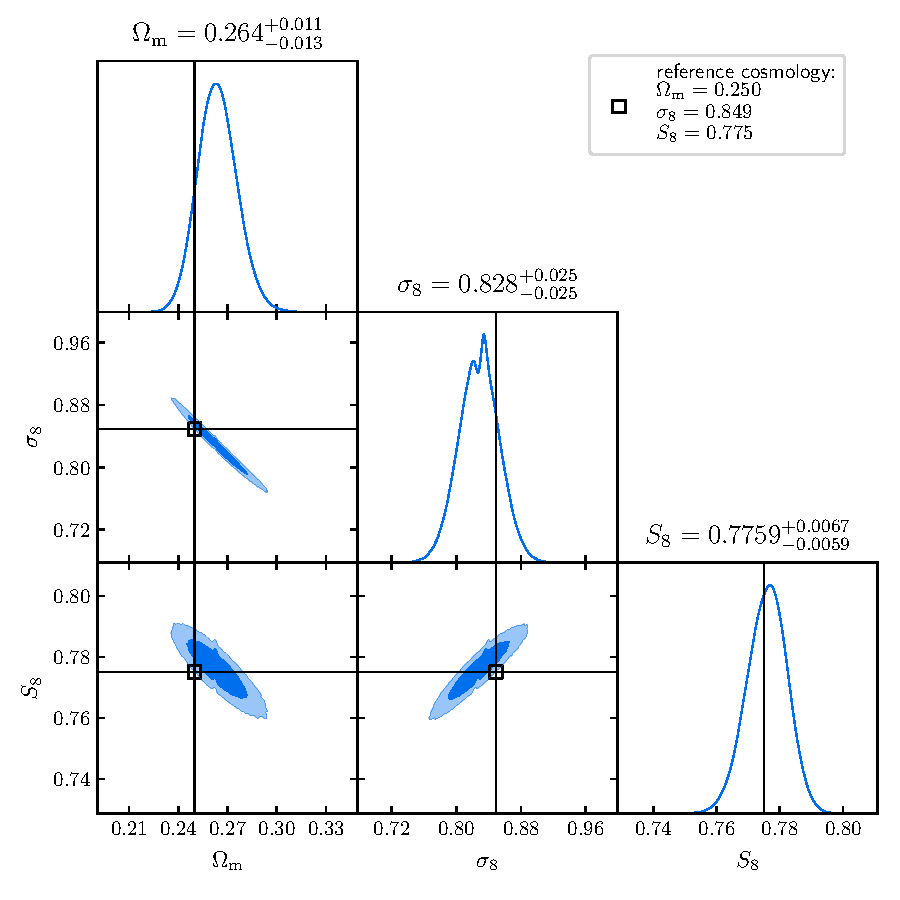
\includegraphics[width=0.7\textwidth]{images/euclid.pdf}
	\caption{Bias in the parameters for a Euclid-like Survey.}
	\label{fig:mcmc_euclid}
\end{figure}  
\todo{Put both in one plot? Maybe put reference MC simulation where $\xi_\pm$ was not changed?}
\end{appendix}
\end{document}
%
